ATTACHMENT IV

DEFINITION OF ``TILES'' WITH TIME-DEPENDENT ATTRIBUTES

\emph{How to code ``tiles'' with Product definition templates 4.55 and 4.56}

The land surface model is evolving and growing more complex. More complex descriptive capabilities are needed to properly describe the representation of land cover types in state-of-the-art weather and climate models.

This includes the sub-grid scale tiling to represent surface heterogeneity. Each grid box with sub-grid variability is divided into a number of tiles, each representing a single surface type.

The use of PDT 4.53 and 4.54 for partitioned parameters implies that for every chosen partition PN(1), PN(2), \ldots, PN(NP) a GRIB message exists. All NP partitions are linked by the normalization formula.

The GRIB code representation of this tile approach takes into account the possibility to encode:

(1) Only the {dominating} tiles, which could differ from grid box to grid box;

(2) Tile attributes, considering that tile fractions can be modified according to Code table 4.241\\
(for example, snow-covered).

Point (1) implies that every grid box has its own subset of tile classes from the land-use table.

Point (2) allows for the differentiation of tile attributes, the {temporal component} of this approach.

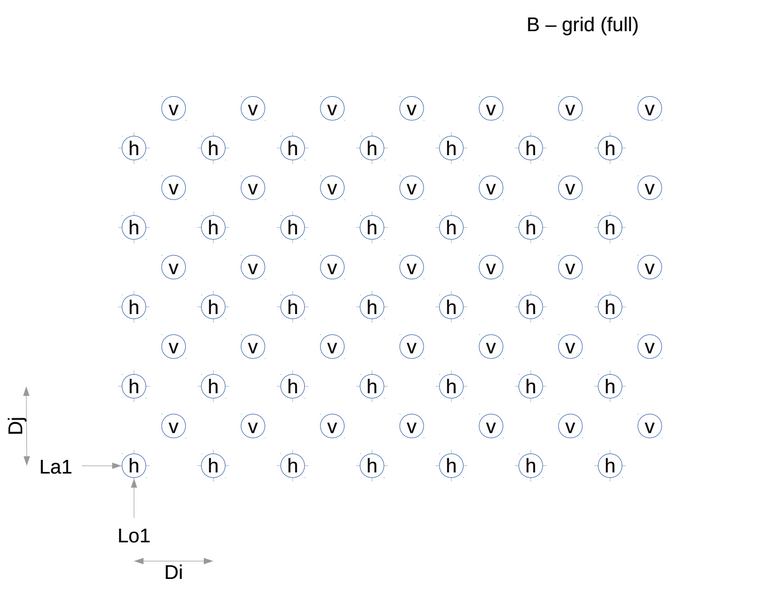
\includegraphics{../tex/extracted-media/media/image1.wmf}The fractions \(f_{i}\) of these \emph{N} (dominant) classes and their attributes are subject to a normalization formula:

In detail, the model grid box is regarded as consisting of a prescribed number of surface types (tiles).

The fractional area of each tile is either given by the geospatial surface data or by one or more prescribed tile attributes (for example, snow-free and snow-covered). It is important to note that in contrast to the geospatial surface data, the tile attributes according to Code table 4.241 could be time dependent.

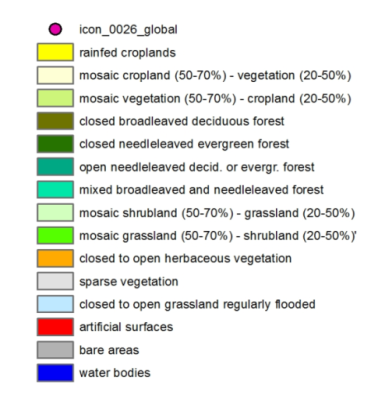
\includegraphics[width=1.6875in,height=1.79583in]{../tex/extracted-media/media/image2.png}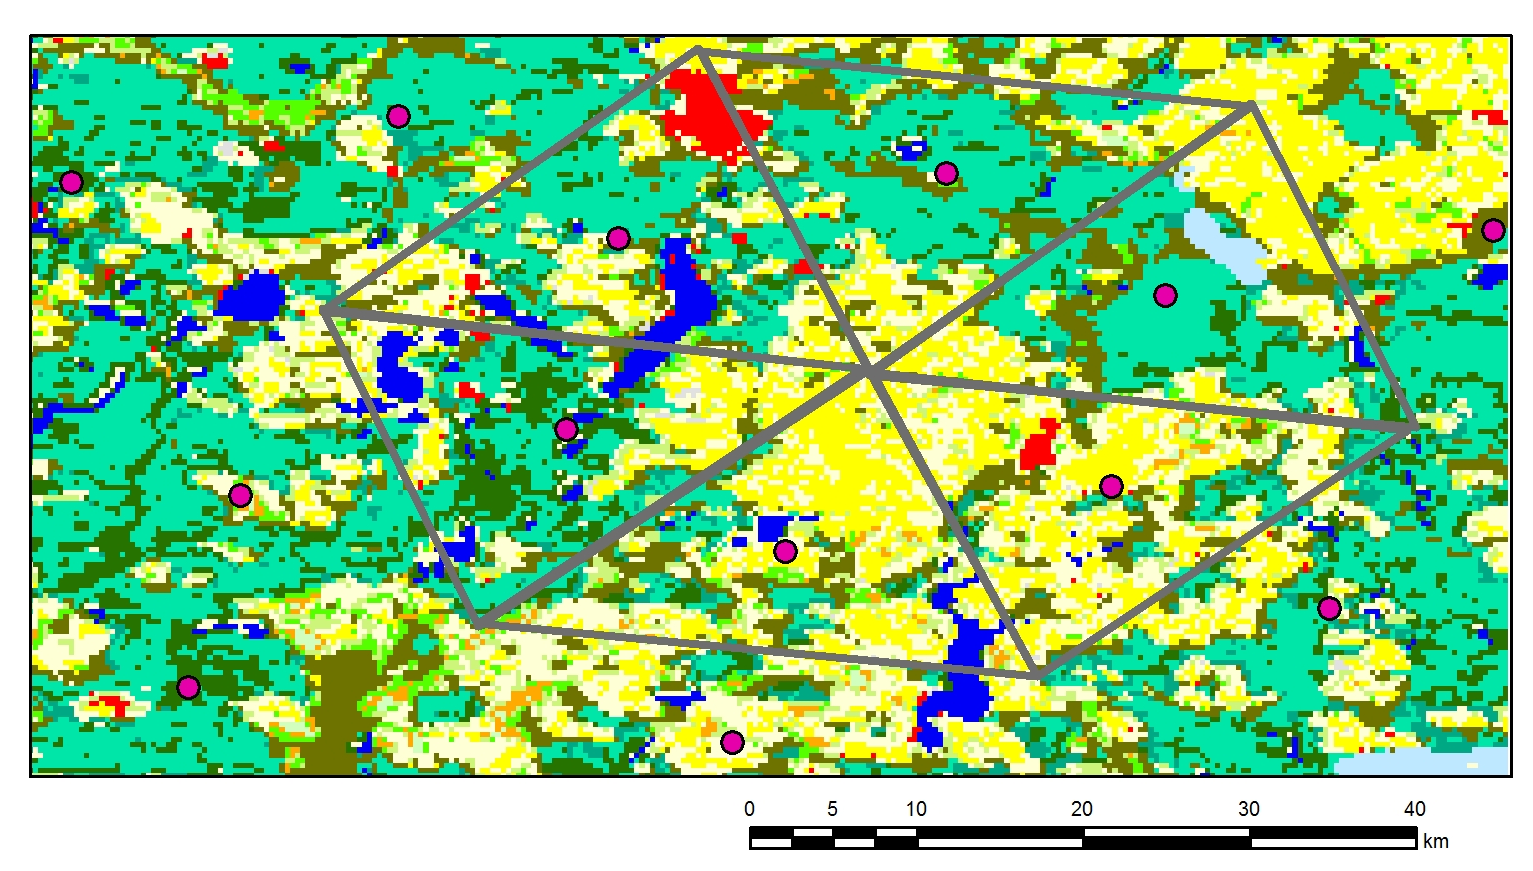
\includegraphics[width=6.67153in,height=3.30764in]{../tex/extracted-media/media/image4.png}

\emph{Figure 1. Generation of the dominating tile structure for NUT=3 of a heterogeneous land surface. The outer circle shows the fractional areas covered by the respective land cover classes for a given grid cell. The inner circle shows the selected dominating tiles. Please note the rescaling of the fractional areas performed in the inner circle.}

Given the number of land-use surface types from the geospatial land-use data table in a particular grid box, the approach recognizes the most dominant land-use surface types above a prescribed threshold fraction (for example, 5\%) up to the number of used tiles (NUT). Two model grid boxes always use the same number of tiles but could differ in the most dominant land-use surface types (see Figure 1, outer circles). The fraction of the resulting NUT is always rescaled to the total grid box area (see Figure 1, inner circles).

For grid boxes with nearly homogeneous land surface types, the approach recognizes only the single dominant type and the fractional area of the other used tiles is considered as zero (see Figure 2).

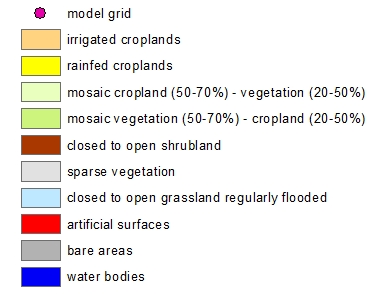
\includegraphics[width=2.2875in,height=2.02014in]{../tex/extracted-media/media/image12.png}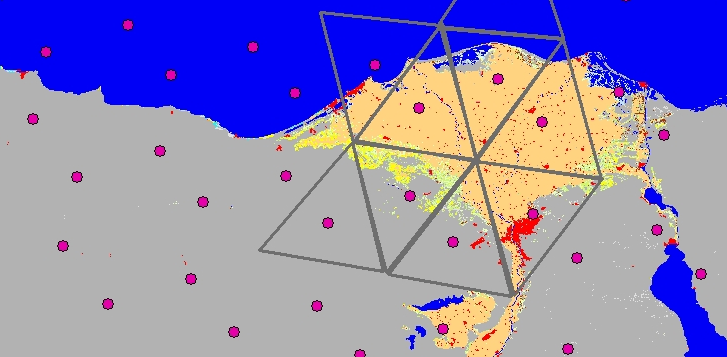
\includegraphics[width=6.94236in,height=3.67222in]{../tex/extracted-media/media/image13.png}

\emph{Figure 2. Generation of the dominating tile structure for NUT=3 of a nearly homogeneous land surface of a coastal region. In this example, area fractions smaller than 5\% are not considered when selecting the dominating tiles.}

The tile attributes considered in this approach allow for a modification of the tile fractions, for example, by a temporal evolution of the snow cover (see Code table 4.241-- Coverage attributes). Therefore, a subset of the land-use classes from the geospatial land-use data table can be considered for tile attributes.

\emph{\\
}

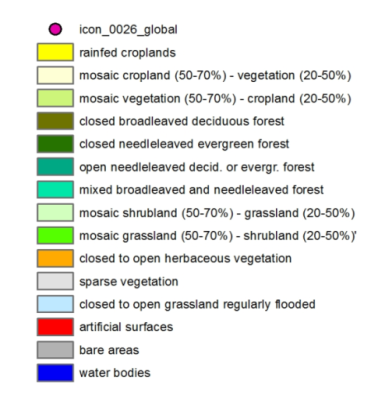
\includegraphics[width=1.6875in,height=1.79583in]{../tex/extracted-media/media/image2.png}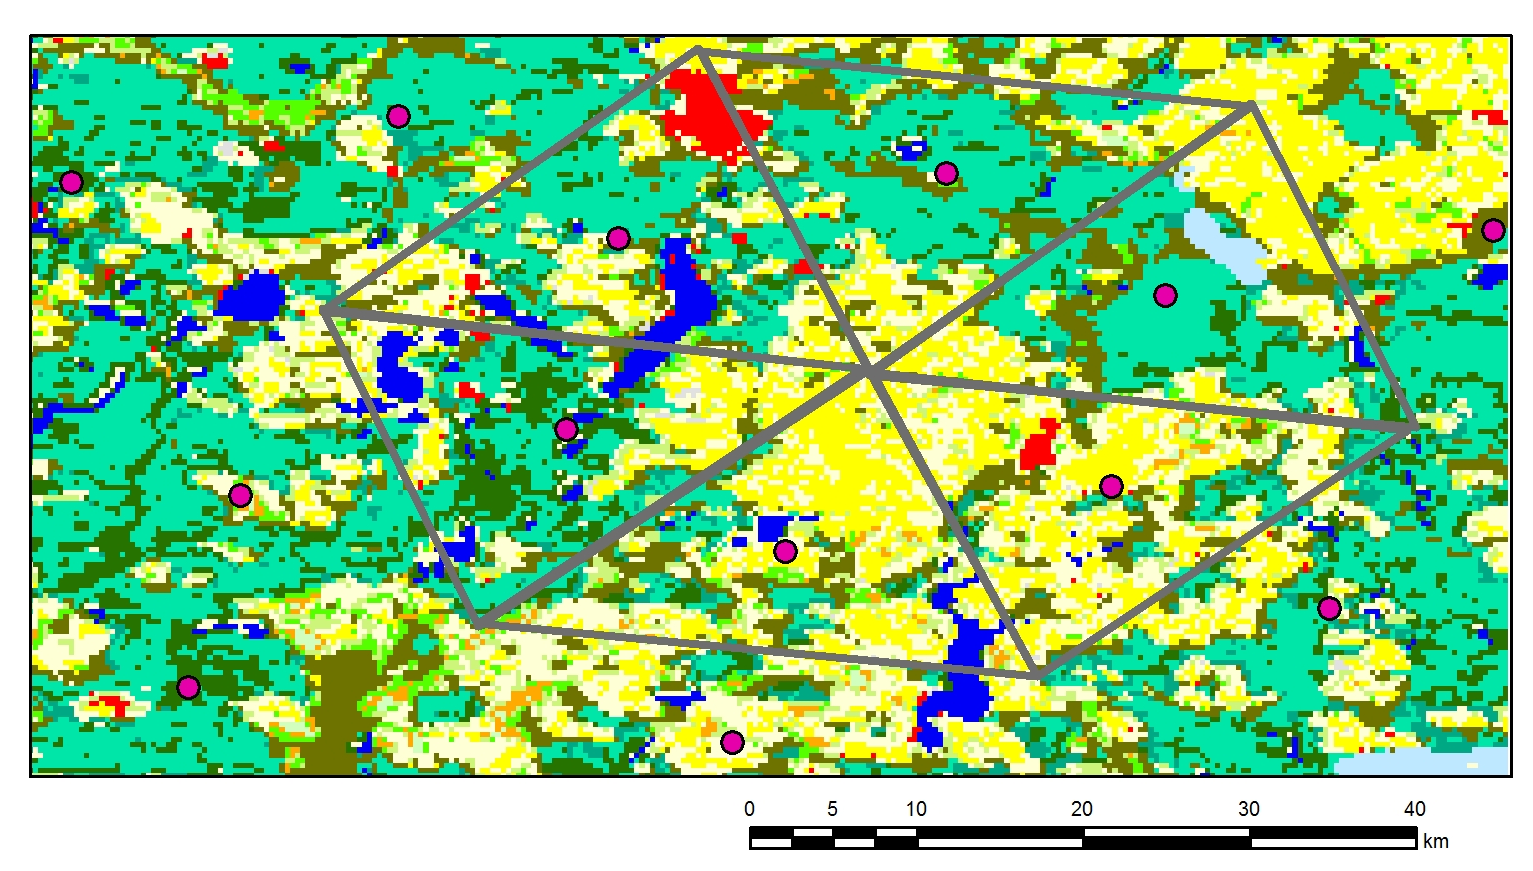
\includegraphics[width=6.77209in,height=3.58605in]{../tex/extracted-media/media/image4.png}

\emph{Figure 3. Generation of the dominating tile structure for NUT=3 with tile attribute ``snow-covered'' of a heterogeneous land surface, partly covered with snow. Dominating tiles are equipped with two attributes where applicable: ``snow-covered'' and ''unmodified''. Shaded areas show the snow-covered tile fractions.}

The tiles used in a particular grid box that belong to the attribute are then divided into fractions of the attribute and fractions of the originating dominating tile (see Figure 3).
